
\chapter{Supply, demand and government policies}

\section{Controls on prices}

\begin{tcolorbox}
  \keyword{price ceiling}
  a legal maximum on the price at which a good can be sold
  \keyword{price floor}
  a legal minimum on the price at which a good can be sold
\end{tcolorbox}

\subsection{How price ceilings affect market outcomes}

\begin{figure}[!ht]
  \centering
  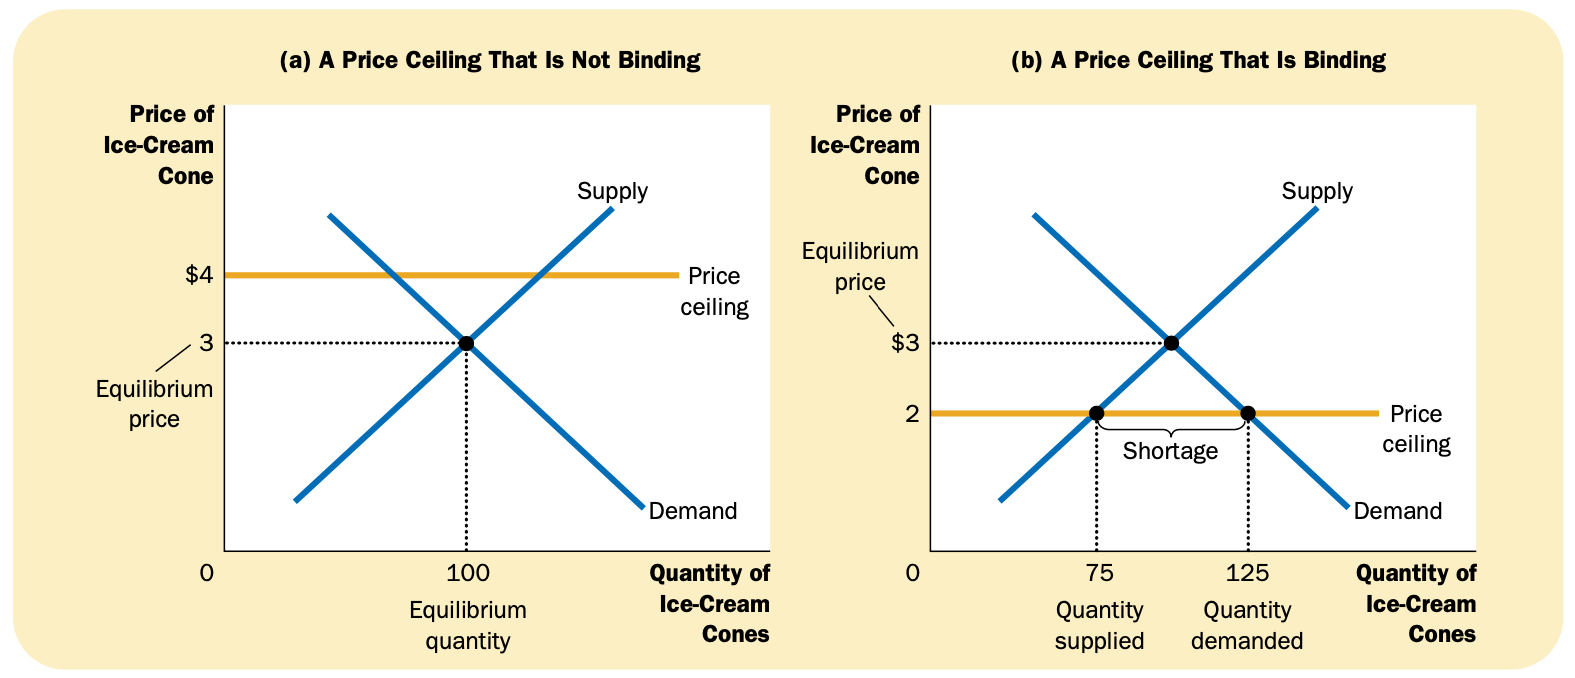
\includegraphics[width=\textwidth]{pics/price-ceiling}
  \caption{A market with price ceiling}
  \label{fig:price-ceiling}
\end{figure}

When the government imposes a binding price ceiling on a competitive market, a shortage of the good arises, and sellers must ration the scarce goods among the large number of potential buyers.


\subsection{How price floors affect market outcomes}


\begin{figure}[!ht]
  \centering
  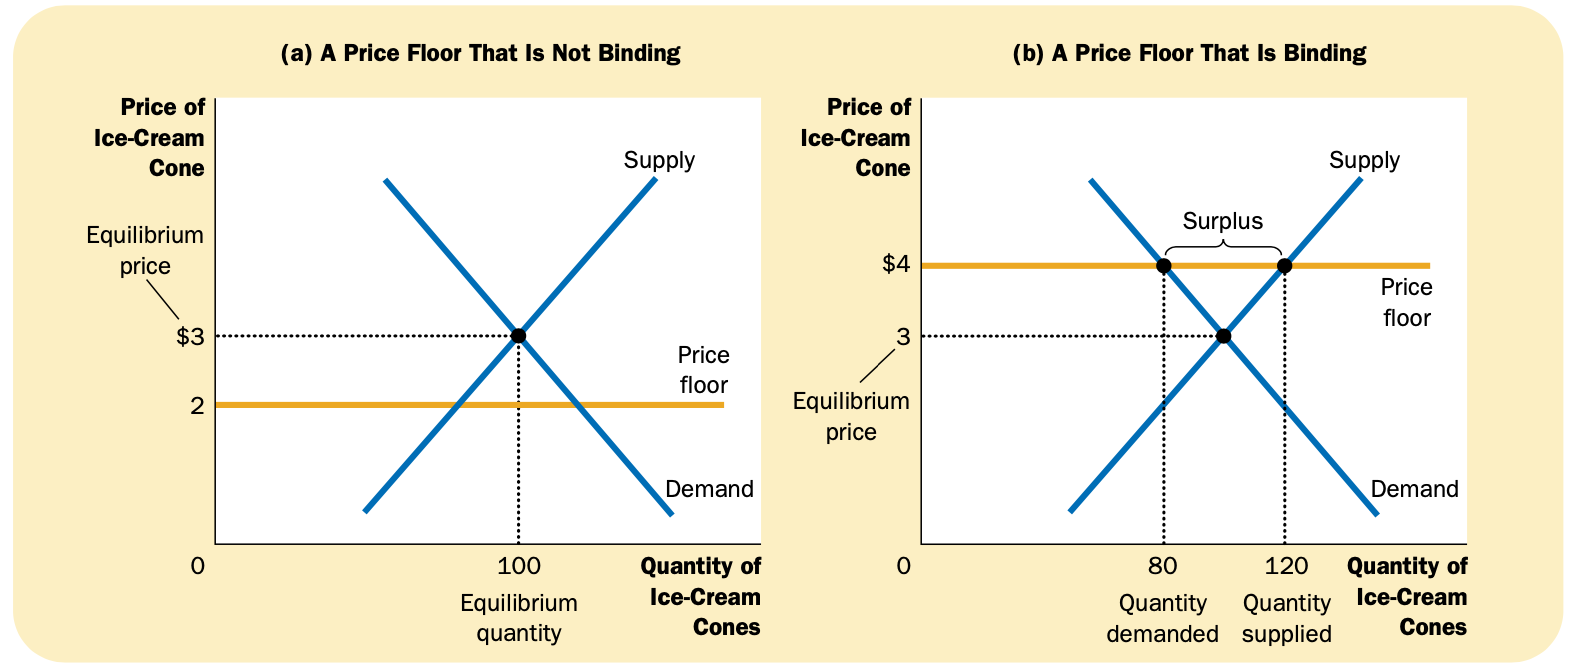
\includegraphics[width=\textwidth]{pics/price-floor}
  \caption{A market with price floor}
  \label{fig:price-floor}
\end{figure}


When the government imposes a binding price floor on a competitive market, a surplus of the good arises.


\section{Taxes}

\begin{tcolorbox}
  \keyword{tax incidence}:
  the study of who bears the burden of taxation
\end{tcolorbox}

\subsection{How taxes on buyers affect market outcomes}

\begin{figure}[!ht]
  \centering
  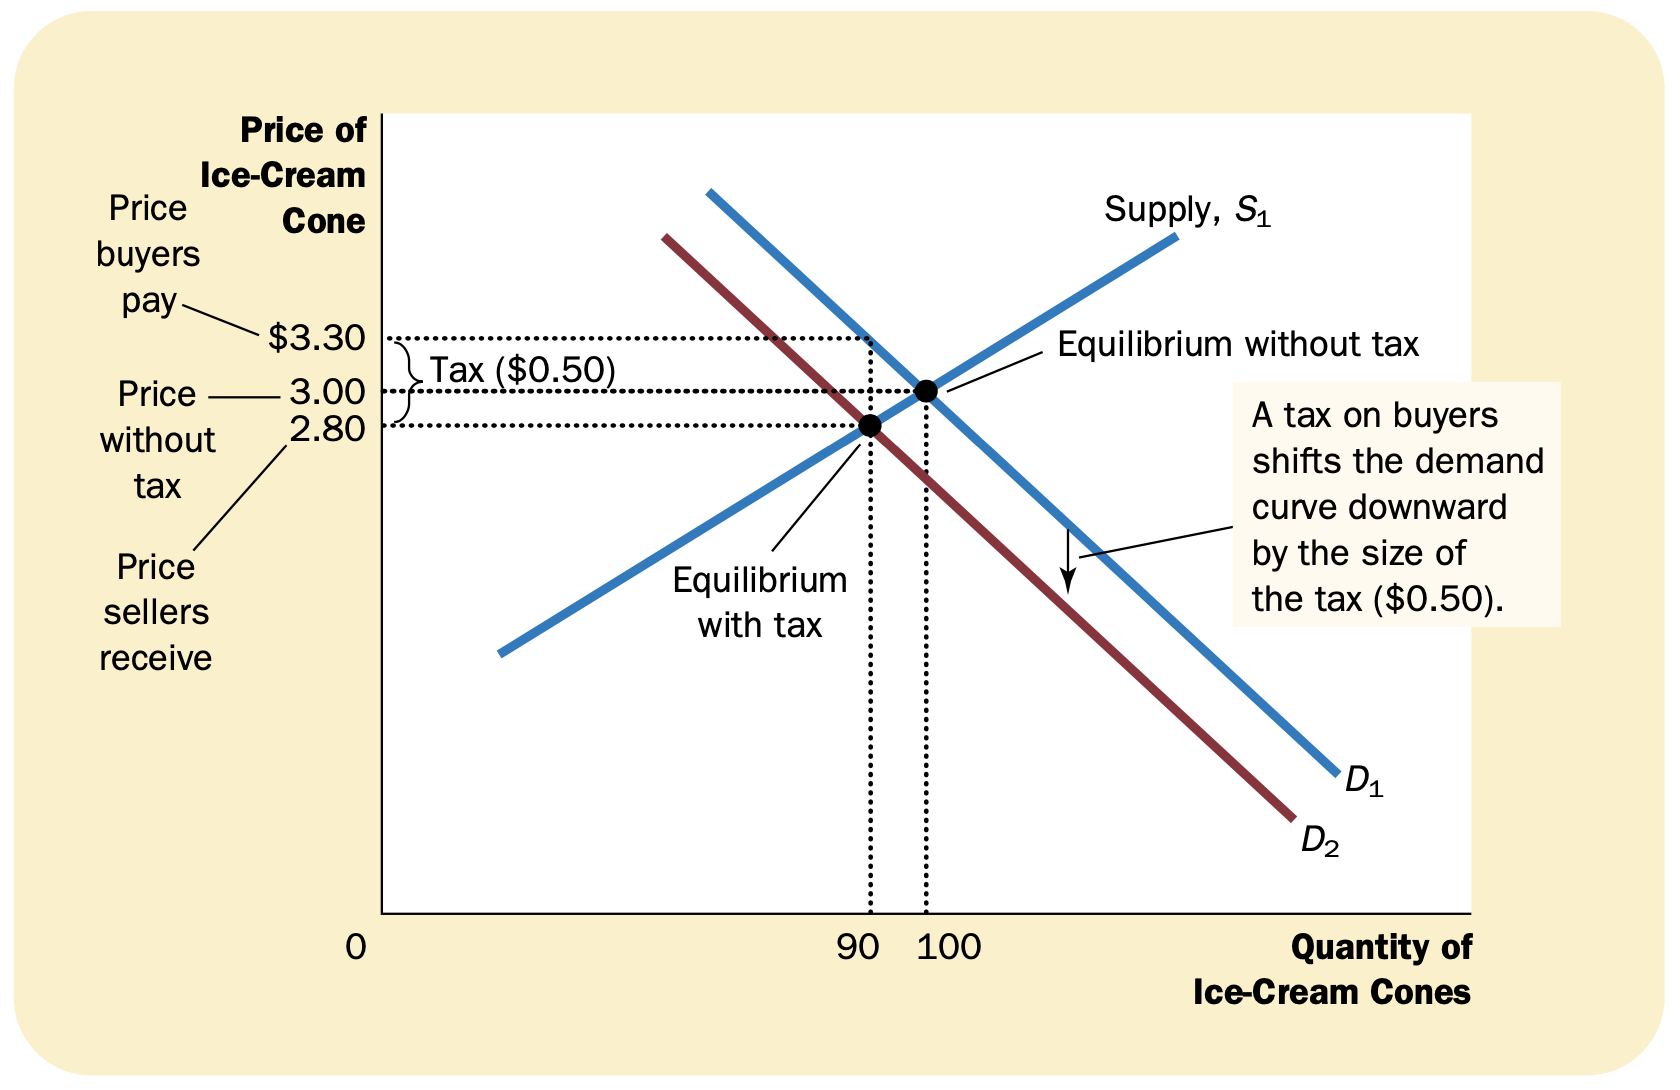
\includegraphics[width=\textwidth]{pics/tax1}
  \caption{A tax on buyers}
  \label{fig:tax1}
\end{figure}

3 steps:
\begin{enumerate}
\item the tax affect the demand curve
\item the demand curve shifts left (or download)
\item the new equilibrium
\end{enumerate}


Two general lessons:
\begin{itemize}
\item Taxes discourage market activity. When a good is taxed, the quantity of the good sold is smaller in the new equilibrium.
\item Buyers and sellers share the burden of taxes. In the new equilibrium, buyers pay more for the good, and sellers receive less.
\end{itemize}

\subsection{How taxes on sellers affect market outcomes}

\begin{figure}[!ht]
  \centering
  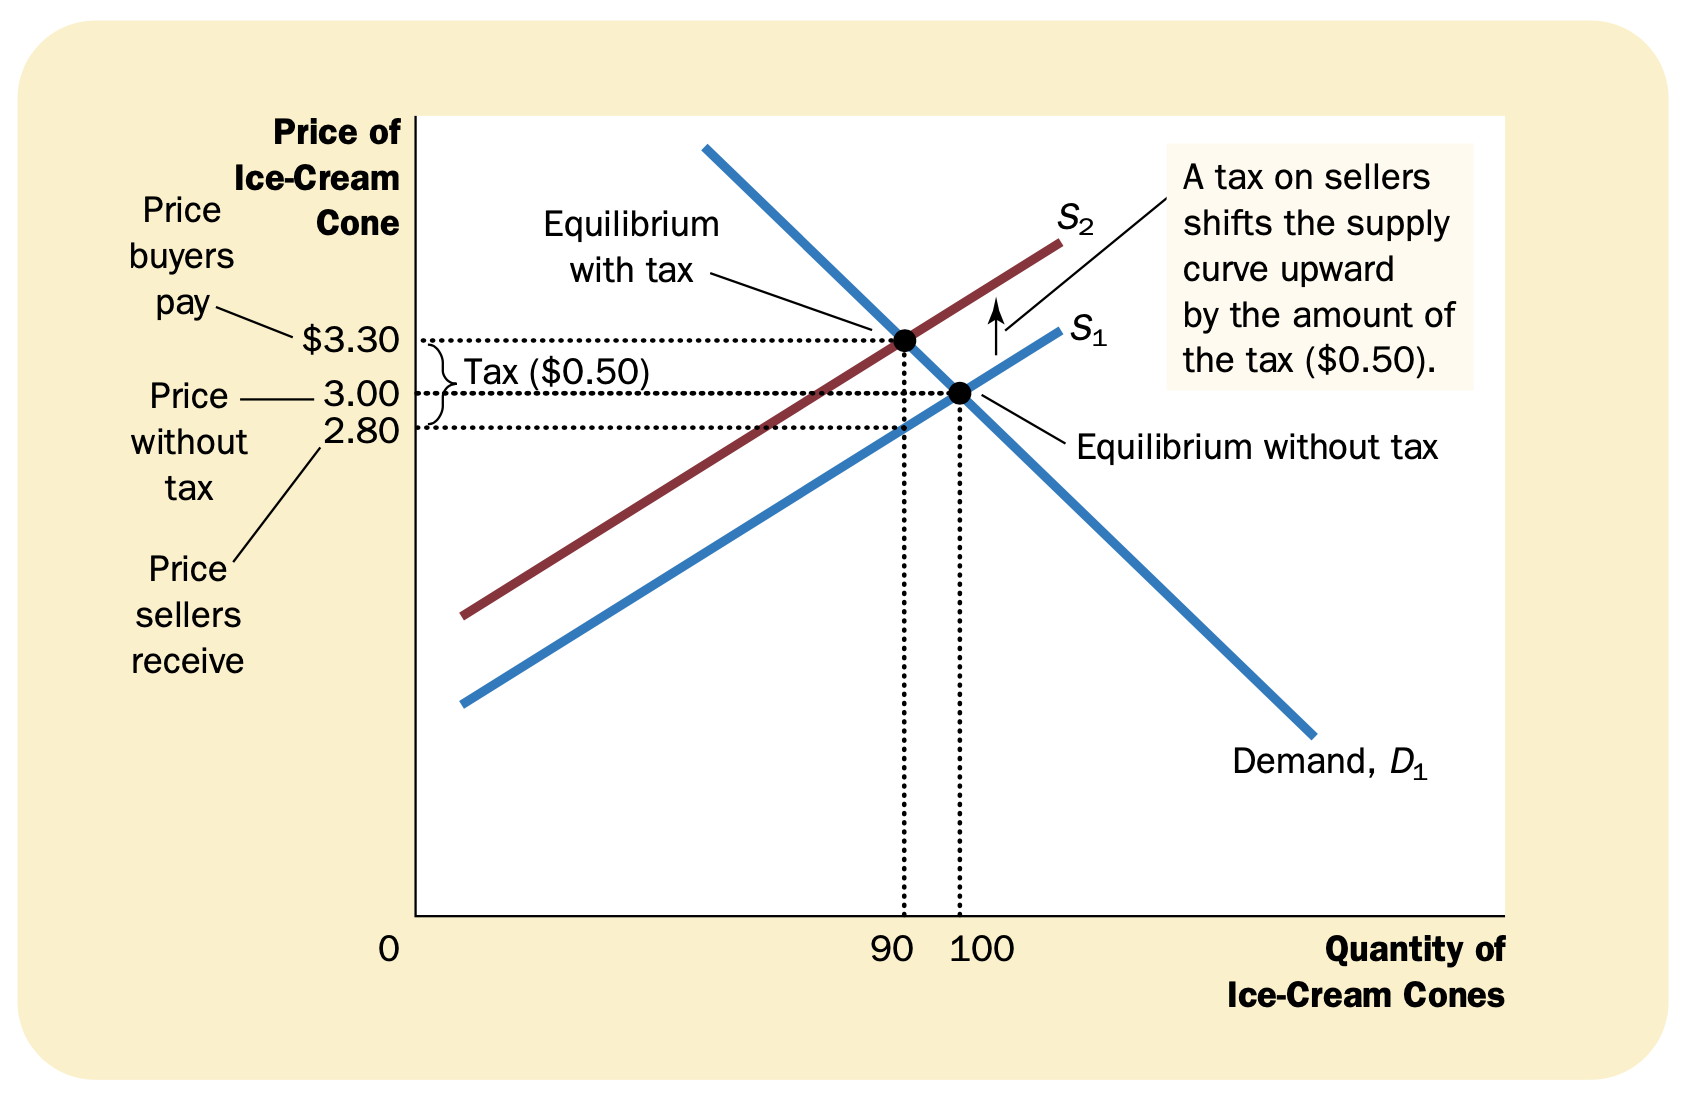
\includegraphics[width=\textwidth]{pics/tax2}
  \caption{A tax on sellers}
  \label{fig:tax2}
\end{figure}


3 steps:
\begin{itemize}
\item the tax affect the supply curve
\item the supply curve shifts left (or up)
\item the new equilibrium
\end{itemize}


Comparing Figure \ref{fig:tax1} and Figure \ref{fig:tax2} leads to a surprising conclusion: Taxes on buyers and taxes on sellers are equivalent.


\subsection{Elasticity and tax incidence}

\begin{figure}[!ht]
  \centering
  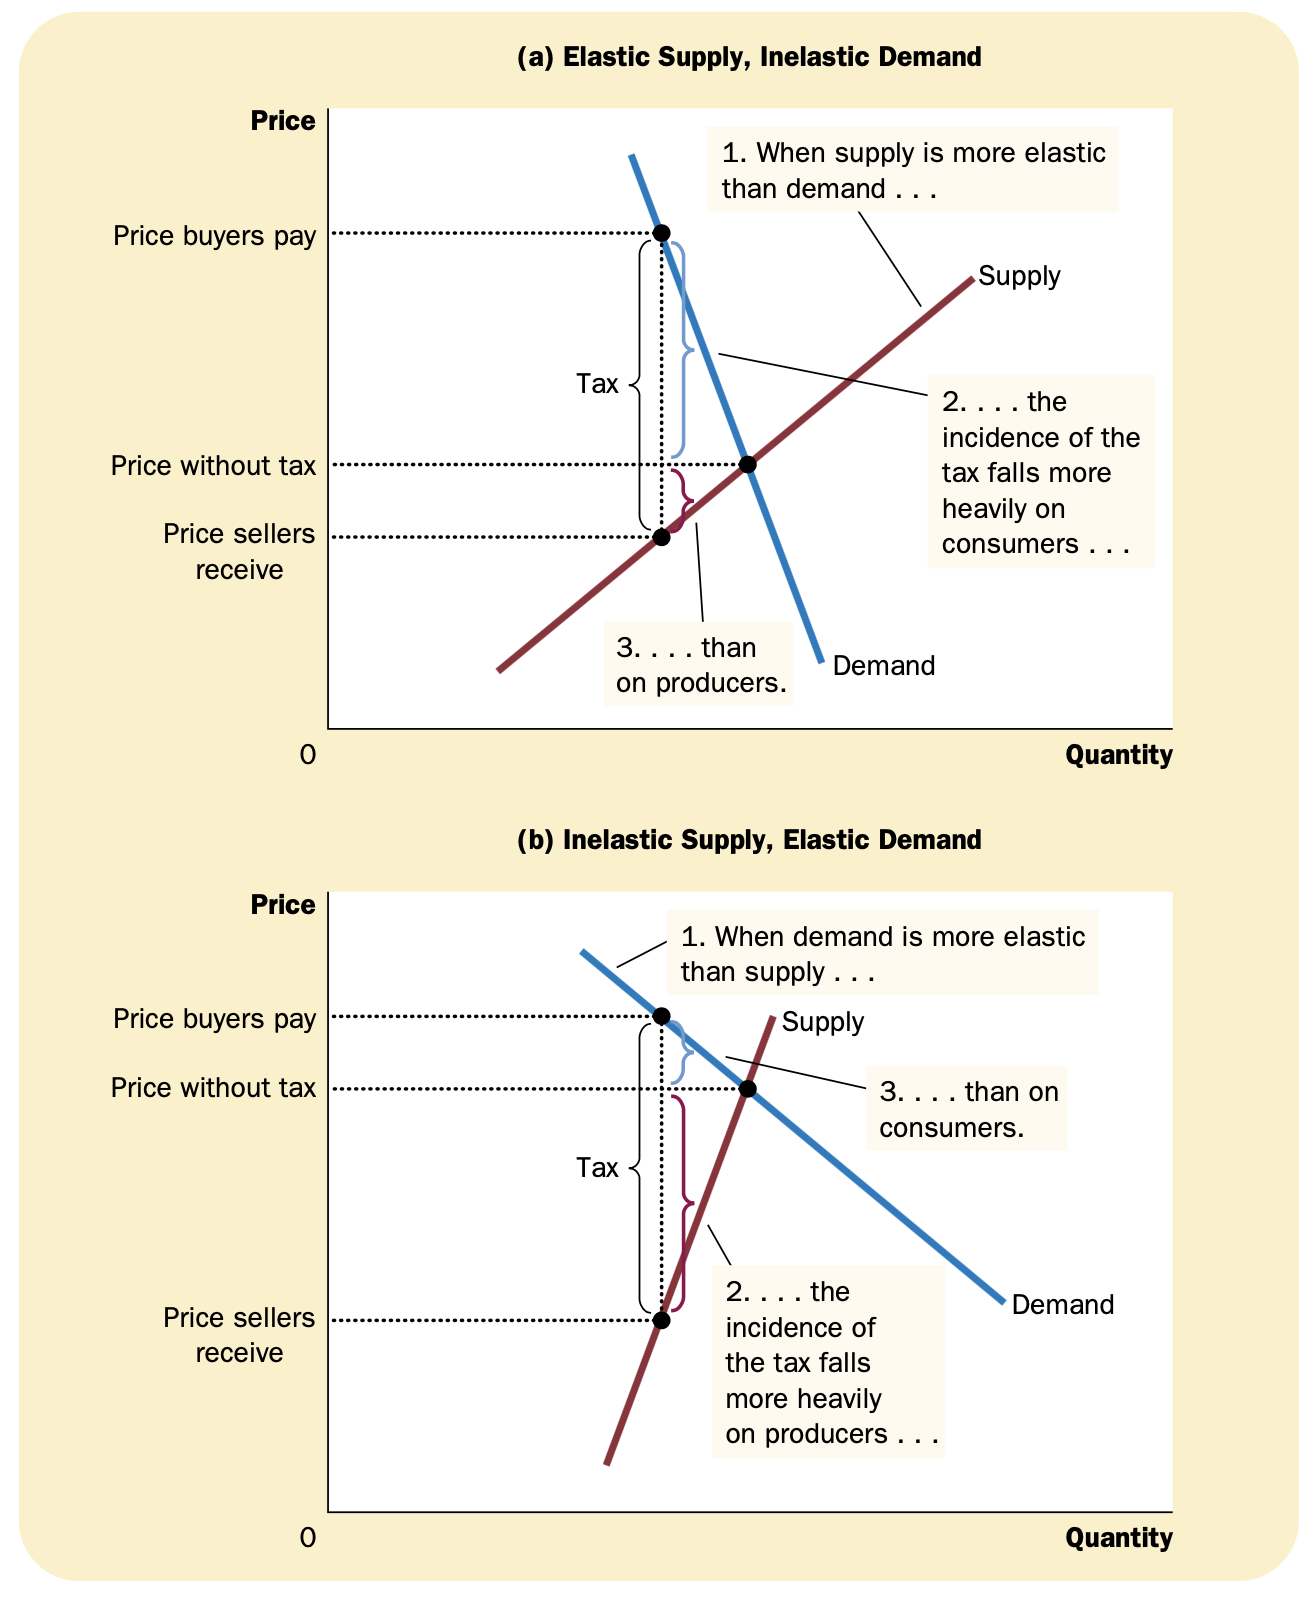
\includegraphics[width=\textwidth]{pics/tax3}
  \caption{How the burden of a tax is divided}
  \label{fig:tax3}
\end{figure}

\keyword{A tax burden falls more heavily on the side of the market that is less elastic.}


Why is this true?

In essence, the elasticity measures the willingness of buyers or sellers to leave the market when conditions become unfavorable.
A small elasticity of demand means that buyers do not have good alternatives to consuming this particular good.
A small elasticity of supply means that sellers do not have good alternatives to producing this particular good.
When the good is taxed, the side of the market with fewer good alternatives cannot easily leave the market and must, therefore, bear more of the burden of the tax.


\begin{tcolorbox}
Most labor economists believe that the supply of labor is much less elastic than the demand.
This means that workers, rather than firms, bear most of the burden of the payroll tax.   
\end{tcolorbox}

